% Build (from docs/paper):  latexmk -xelatex short_paper.tex
\documentclass[10pt,twocolumn]{article}
\usepackage[a4paper,margin=0.8in,columnsep=0.28in]{geometry}
\usepackage{fontspec}
\usepackage{xcolor}
\usepackage{booktabs}
\usepackage{graphicx}
\usepackage{array}
\usepackage{amsmath}
\usepackage[font=small,labelfont=bf,skip=3pt]{caption}
\usepackage[authoryear,round]{natbib}
\usepackage[colorlinks=true,allcolors=blue!50!black]{hyperref}
\usepackage{url}

\setmainfont{Times New Roman}
\setsansfont{Arial}
\newfontfamily\thaifont[Script=Thai,Path=../../assets/fonts/noto/]{NotoSansThai-Regular.ttf}
\newcommand{\thai}[1]{{\thaifont #1}}

% Items that wait for the collaborator's runs (work split W1--W4).
\newcommand{\todo}[1]{\textcolor{red!70!black}{\textbf{[#1]}}}
\newcommand{\code}[1]{\texttt{#1}}

\setlength{\parskip}{0pt}
\setlength{\parindent}{1em}
\setlength{\textfloatsep}{8pt plus 2pt minus 2pt}
\setlength{\floatsep}{6pt plus 2pt minus 2pt}
\setlength{\intextsep}{6pt plus 2pt minus 2pt}
\renewcommand{\arraystretch}{1.08}
\widowpenalty=10000
\clubpenalty=10000

\begin{document}
\twocolumn[
\begin{center}
{\LARGE\bfseries Not Reading, Not Misreading: Where Thai OCR\\[2pt] Vision-Language Models Lose Vowel and Tone Marks\par}
\vspace{8pt}
{\large Draft v1 --- authors to be added\par}
\vspace{2pt}
{\small Pilot results on the ThaiOCRBench calibration split; \todo{red = waits for further runs}\par}
\end{center}
\vspace{4pt}
\begin{center}\begin{minipage}{0.92\textwidth}\small\centerline{\textbf{Abstract}}\vspace{2pt}
Open vision-language models (VLMs) for Thai OCR now read most of a page correctly, yet Thai vowel and tone marks remain a natural worry: one mark changes a word. We ask \emph{where} marks are lost, not only how many. We introduce a mark score that does not charge reading order, charges surplus text, and gives no credit to the copies of a repetition loop. On ThaiOCRBench, Typhoon OCR 1.5 (2B) gets the tone mark wrong in only 0.65\% of the places where it reads the base consonant correctly, and, given the correct preceding text, it chooses the tone mark correctly 98.8\% of the time even without the image. Most marks it loses are never read: lines are absent, spans are missing, or the output is consumed by a loop. Among training-free decoders, stopping at a detected loop leaves every non-looping output unchanged and raises mark F1 by 0.8 points for Typhoon and 10.8 points for a 0.9B Thai model, whereas a repetition penalty lowers F1 on pages that do not loop, and subtracting the language prior removes correct tone marks. \todo{Other models (W1--W3) and a locked-split confirmation (W4) are pending.} All results are preliminary: one benchmark, a calibration split, and rules written after the data were seen.
\end{minipage}\end{center}
\vspace{6pt}
]

\section{Introduction}
Thai is written with a line of consonants and marks stacked above and below it: upper vowels, lower vowels, and four tone marks. One mark can change the meaning and the pronunciation of a word (\thai{ข่าว} ``news'' against \thai{ข้าว} ``rice''), so a transcription that drops or swaps a mark is wrong for a reader even when almost every character is right. Yet Thai OCR is scored with whole-text measures: n-gram overlap and normalized edit distance in ThaiOCRBench \citep{nonesung2025thaiocrbench}, and character error rate elsewhere. These numbers do not say whether the marks are the problem, and sequence-level scores also charge a model for reading a page's columns in a different order than the reference.

Open VLMs trained for Thai OCR are now available \citep{nonesung2026typhoonocr,nectec2026pathumma,pipatanakul2026synthetic}. They raise a practical question: when such a model gets a Thai mark wrong, what went wrong? One possibility is that the visual evidence for a small mark is lost or too weak. Another is that the model's language prior overrides that evidence. A third is that the mark is never read at all, because the model skipped the line, failed to find the text, or fell into a repetition loop. The remedies differ. If the image is the problem, one re-reads or zooms. If the prior is the problem, one subtracts the prior, as contrastive decoding does \citep{leng2024vcd,favero2024m3id}. If the text is never read, the fix lies in decoding or in finding the text.

We study this on ThaiOCRBench with Typhoon OCR 1.5 and four other open checkpoints, on full-page OCR and text recognition. We make three contributions.
\begin{enumerate}\itemsep0pt\topsep2pt
\item \textbf{A mark score that does not charge reading order} (Section~\ref{sec:metric}). It scores upper vowels, lower vowels and tone marks per reference line, wherever that line appears in the output; it charges surplus text; and it gives no credit to copies of a repetition loop.
\item \textbf{A diagnosis of where marks are lost} (Section~\ref{sec:where}). For Typhoon, a correctly read consonant is followed by a wrong tone mark only 0.65\% of the time, and with the correct preceding text the tone mark is chosen correctly 98.8\% of the time without the image. The marks that are lost are mostly not read at all. \todo{W1/W3: the same diagnosis for the other models.}
\item \textbf{What training-free decoding does to marks} (Section~\ref{sec:decoding}). Stopping at a detected loop changes no non-looping output and raises mark F1; a repetition penalty lowers F1 on non-looping pages; subtracting the language prior removes correct tone marks. \todo{W4: confirmation on the locked split.}
\end{enumerate}
Taken together, for the models studied the remaining mark errors of a strong Thai OCR model sit upstream of the mark itself. The useful levers are in decoding and in finding text, not in seeing a tone mark more sharply.

\section{Related Work}
\paragraph{Thai OCR with VLMs.} ThaiOCRBench \citep{nonesung2025thaiocrbench} evaluates proprietary and open VLMs on Thai document tasks, including full-page OCR and text recognition, with n-gram overlap and edit-distance measures (BLEU, METEOR, F1, normalized Levenshtein; ANLS for text recognition). Its introduction names stacked diacritics as a Thai difficulty, but no score isolates the marks. Open Thai OCR models have since appeared: Typhoon OCR \citep{nonesung2026typhoonocr}, a full fine-tune of Qwen3-VL-2B \citep{bai2025qwen3vl} in version 1.5, whose authors list infographics as an area for improvement; Pathumma-llm-vision 3.0 \citep{nectec2026pathumma}, another Qwen3-VL-2B fine-tune; and wayu-paxa-ocr-zero \citep{pipatanakul2026synthetic}, a fine-tune of PaddleOCR-VL \citep{cui2025paddleocrvl} on synthetic Thai pages. Each reports aggregate accuracy; we ask where marks are lost.

\paragraph{Diacritics in OCR.} Diacritic-heavy scripts are known to be hard for OCR. Post-OCR correction has been proposed for Vietnamese diacritics \citep{do2025reference}, and Arabic OCR evaluations treat diacritized text as a separate condition \citep{elsafty2025arabic}. We know of no work that scores Thai marks separately from reading order and surplus text.

\paragraph{Repetition and omission.} Likelihood-maximizing decoding yields repetitive text \citep{holtzman2020curious}, and document OCR models degenerate the same way. Nougat reports pages where the model repeats a sentence and stops generation when a logit-variance signal falls \citep{blecher2024nougat}; olmOCR retries at a higher temperature \citep{poznanski2025olmocr}; the PaddleOCR-VL pipeline truncates repetitive output after decoding \citep{paddlex2025truncate}; DeepSeek-OCR's released code bans repeated n-grams within a window \citep{deepseekocr2025code,wei2025deepseekocr}. CC-OCR measures repetition as OCR hallucination \citep{yang2025ccocr}. These works treat repetition as something to detect or avoid; we measure what each remedy costs the marks on pages that do not loop, including the repetition penalty of CTRL \citep{keskar2019ctrl} that some OCR packages ship by default.

\paragraph{Language priors and training-free decoding.} Contrastive decoding reduces VLM hallucination by down-weighting what the model would predict without, or with degraded, visual input: VCD \citep{leng2024vcd}, M3ID \citep{favero2024m3id} and PAI \citep{liu2024pai}. They assume the language prior is the problem; for Thai tone marks we find the prior is usually right. Our variants are reimplementations, called ``M3ID-form'' and ``PAI-style''. Speculative decoding \citep{leviathan2023speculative}, here with prompt-lookup drafts \citep{saxena2023pld}, speeds up decoding without changing its output in exact arithmetic.

\section{Scoring Marks Without Charging Reading Order}\label{sec:metric}
The \emph{marks} are the six upper vowels (\thai{ั ิ ี ึ ื ็}), the two lower vowels (\thai{ุ ู}) and the four tone marks (\thai{่ ้ ๊ ๋}). A full-page reference has several lines, and a model may read the columns of a page in another order than the reference. A global alignment then calls correctly read marks wrong.

\paragraph{Definition.} Reference lines of at least eight characters are processed longest first. For each, we find the stretch of the output, with characters already claimed masked, that aligns to it at under 40\% character error rate, credit the marks that match, and claim the stretch, so one output stretch never credits two lines. Lines left unmatched are aligned globally, in reference order, against the output with every claimed character removed; without this step, marks inside a poorly read line were dropped (our first version failed its check against the base model). Recall is the credited marks over the reference marks. Precision is the credited marks over \emph{all} marks in the output, so surplus text is charged. F1 is micro-averaged over items.

\paragraph{Repeat-aware variant.} In this variant, credit is computed on the output after reducing every loop run to one copy (a run is a 4--400 character unit with a letter, repeated exactly at least eight times, or six for units of 50+ characters). Precision still counts every mark of the full output, so the copies are charged but cannot earn recall. It was added after a collaborator noticed that the alignment lined up 434 copies of a repeated unit with common syllables across the reference. With no loop the two scores are identical.

\paragraph{Checks.} Reading two runs of the same page one after the other scores far below the better single run; the base model's recall stays within 0.3 points of the global alignment in every cell; and Typhoon's full-page recall rises by 1.6--1.8 points when order is not charged. Charging reading order alone lowers Typhoon's full-page mark F1 from 94.9 to 93.1 (BQ; 95.3 to 93.7 for TC). The base model is barely affected.

\section{Setup}\label{sec:setup}
\paragraph{Data.} ThaiOCRBench \citep{nonesung2025thaiocrbench} test split, two tasks: full-page OCR and text recognition. We use a seeded 30\% calibration split stratified by task and category: 69 full-page and 109 text-recognition items. A locked 70\% split is unopened. Per-item outputs and scores are reported; no benchmark image is redistributed.

\paragraph{Models.} Typhoon OCR 1.5 (2B) and its base Qwen3-VL-2B; Qwen3-VL-4B; PaddleOCR-VL-1.6 and wayu-paxa-ocr-zero (``Wayu''), both 0.9B region recognizers used here also on full pages, which is off their design. Every checkpoint is pinned by revision (Appendix). We use the Apache-2.0-only revision of Typhoon.

\paragraph{Prompts and decoding.} \textbf{BQ} is the benchmark's own question for each item; \textbf{TC} is the prompt recommended on Typhoon's model card. Paddle and Wayu use their \code{OCR:} prompt. Decoding is greedy, at most 3,072 new tokens, fp16 on Kaggle T4 GPUs. Each result below is one run. Outputs are reduced to plain text (markup removed) before scoring. We report BQ as primary and TC as secondary.

\paragraph{Statistics.} Intervals are 95\% bootstrap intervals over items. All results are \emph{preliminary pilot} results on the calibration split; several decoding rules were written after the same split was seen, and we flag each.

\section{Where Marks Are Lost}\label{sec:where}
\subsection{Five models}
\begin{figure}[t]
\centering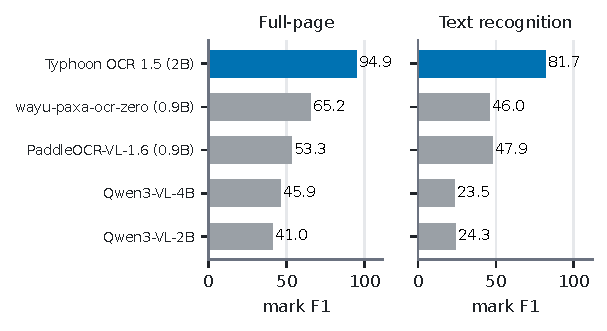
\includegraphics[width=\columnwidth]{figures/fig_models.pdf}
\caption{Mark F1 (order-free, BQ; \code{OCR:} for the two 0.9B models) on the calibration split. Typhoon is highest on both tasks.}\label{fig:models}
\end{figure}
Typhoon scores 94.9 mark F1 on full pages and 81.7 on text recognition, far above the other four (Figure~\ref{fig:models}, Table~\ref{tab:models}). Against Typhoon, Wayu is lower by 29.6 points [39.9, 19.2] on full pages. Doubling the base model's size changes full-page F1 by +5.0 [$-$4.0, +14.1], and its tone error stays at about 9.4--9.9\%. Typhoon's median per-page character error rate is 2.8\%. These models are compared as shipped, with unequal visual-token budgets. Among the models measured, Typhoon is the best here; Pathumma-llm-vision 3.0 reports higher ThaiOCRBench scores on text recognition and overall \citep{nectec2026pathumma}, and we have not measured it. \todo{W2: Pathumma-llm-vision 3.0 and further models.}

\begin{table}[t]
\centering\small
\begin{tabular}{@{}l rrr rr@{}}
\toprule
 & \multicolumn{3}{c}{Full-page} & \multicolumn{2}{c}{Text rec.}\\
\cmidrule(lr){2-4}\cmidrule(l){5-6}
Model & F1 & tone err.\ & trunc.\ & F1 & trunc.\\
\midrule
Typhoon OCR 1.5 & \textbf{94.9} & 0.65 & 2.9 & \textbf{81.7} & 0.9\\
Wayu & 65.2 & 5.27 & 26.1 & 46.0 & 20.2\\
PaddleOCR-VL-1.6 & 53.3 & 14.57 & 39.1 & 47.9 & 14.7\\
Qwen3-VL-4B & 45.9 & 9.89 & 27.5 & 23.5 & 11.9\\
Qwen3-VL-2B & 41.0 & 9.41 & 43.5 & 24.3 & 14.7\\
\bottomrule
\end{tabular}
\caption{Order-free mark F1, tone-mark error given a correctly read consonant (\%), and outputs that reached the token limit (\%). Calibration split, primary prompts.}\label{tab:models}
\end{table}

\paragraph{Loop copies earned recall.} The repeat-aware score changes Typhoon by at most 0.2 points but lowers the base model's full-page F1 (BQ) from 41.0 to 34.4 and its recall from 65.0 to 54.6: about a sixth of the marks the order-free score credited to it came from loop copies (Table~\ref{tab:repeat}). We read back every stripped run: all 126 reached the token limit, the shortest has 15 copies, and no ordinary text was stripped.

\begin{table}[t]
\centering\small
\begin{tabular}{@{}l rrr rrr@{}}
\toprule
 & \multicolumn{3}{c}{order-free} & \multicolumn{3}{c}{repeat-aware}\\
\cmidrule(lr){2-4}\cmidrule(l){5-7}
Full-page, BQ & R & P & F1 & R & P & F1\\
\midrule
Typhoon & 96.1 & 93.7 & 94.9 & 96.1 & 93.6 & 94.8\\
Qwen3-VL-2B & 65.0 & 29.9 & 41.0 & 54.6 & 25.1 & 34.4\\
\bottomrule
\end{tabular}
\caption{Recall, precision and F1 (\%) with and without credit for loop copies.}\label{tab:repeat}
\end{table}

\subsection{Typhoon's lost marks are mostly not read}
Of all reference marks on full pages, Typhoon gets 6.2\% (BQ) and 7.1\% (TC) wrong. We attribute each to one cause automatically (Figure~\ref{fig:causes}): the line is read in another order (a stretch of the output matches it at under 20\% character error rate, for lines of at least eight characters); the whole line is absent; a span is missing inside a kept line; or the mark is misread. Whole lines absent account for 2.3\% (BQ) and 2.9\% (TC) of marks, spans missing for 0.7\% and 0.8\%, and misreads for 1.5\% and 2.4\%. Reading order alone accounts for 1.6\% and 0.9\%, which is not an error of reading. Opening the raw outputs, the absent lines are mainly text inside infographics and charts, inset advertisements, and titles and page furniture, where Typhoon writes an image placeholder; this agrees with its authors' note on infographics \citep{nonesung2026typhoonocr}. The base model, by contrast, loses about 41\% of marks. The attribution is automatic; page images were checked only for the six pages that hold most absent marks. \todo{W1: attribution for the other models.}

\begin{figure}[t]
\centering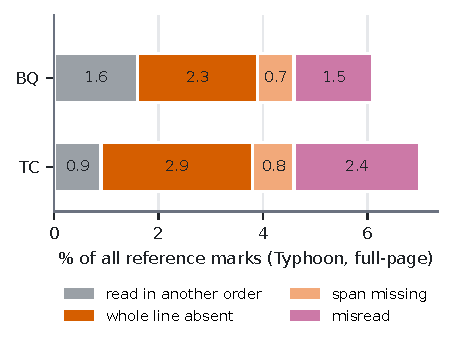
\includegraphics[width=0.96\columnwidth]{figures/fig_causes.pdf}
\caption{Where Typhoon's full-page mark loss goes, as a share of all reference marks.}\label{fig:causes}
\end{figure}

\subsection{Given the right context, the prior is already right}
In a forced-choice test we give the model the correct text up to a mark site and let it score the legal variants of that mark with and without the image (fp32, in-context tokenization). Typhoon chooses the correct tone mark on full pages 99.7\% of the time with the image and 98.8\% without it; the base model, 98.1\% and 98.9\% (Figure~\ref{fig:prior}, left). The image adds 0.9 points for Typhoon and subtracts 0.8 for the base. This is a forced choice with correct context and not free generation. In this pair the specialized model's image gain is larger, not smaller, than the base's; we do not generalize it. \todo{W3: the same test for Pathumma and Qwen3-VL-4B.}

\paragraph{Confidence.} Typhoon's own token probability locates its mark errors: the lowest token probability inside a cluster separates misread marks from correct ones with an AUROC of 0.918 (BQ) and 0.935 (TC), on the model's own greedy output.

\begin{figure}[t]
\centering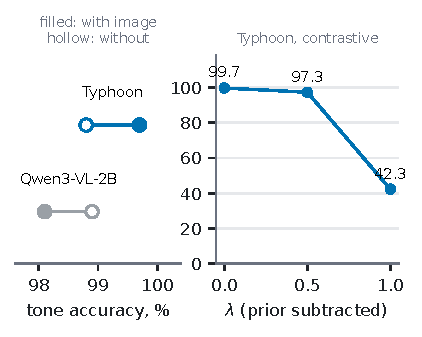
\includegraphics[width=\columnwidth]{figures/fig_prior.pdf}
\caption{Left: tone accuracy at the registered sites with and without the image. Right: Typhoon's accuracy when the no-image score is subtracted with weight $\lambda$.}\label{fig:prior}
\end{figure}

\section{Training-Free Decoding and Marks}\label{sec:decoding}
\subsection{Loops are rare and costly}
Of 356 Typhoon outputs (BQ and TC, both tasks), 11 loop. Two to five looping pages hold 68--76\% of all surplus marks in a cell; without them, full-page F1 (BQ) would be 97.4 rather than 94.9 (this is a ceiling from removing those pages, not a method).

\subsection{Three ways to handle a loop}
We compare three decoders for Typhoon against greedy decoding (Figure~\ref{fig:decoders}; BQ full pages):
\begin{itemize}\itemsep0pt\topsep2pt
\item \textbf{Repetition penalty 1.1}, the anti-repetition setting of Typhoon's own package, using the penalty of CTRL \citep{keskar2019ctrl}.
\item \textbf{n-gram blocking} as in DeepSeek-OCR's code: no repeated 30-gram within 90 tokens.
\item \textbf{Stop at a detected loop}: when a unit repeats eight times (six for units of 50+ characters), decoding stops at the first copy. Greedy decoding is prefix-deterministic, so we compute the cut offline from complete greedy outputs; a decode-time implementation has not yet been verified against it.
\end{itemize}
\begin{figure}[t]
\centering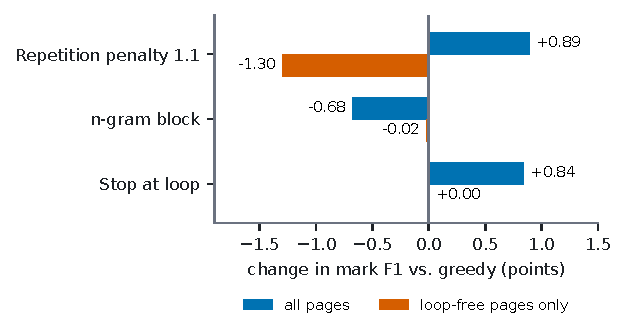
\includegraphics[width=\columnwidth]{figures/fig_decoders.pdf}
\caption{Change in full-page mark F1 against greedy decoding (Typhoon, BQ) on all pages and on pages that do not loop.}\label{fig:decoders}
\end{figure}

\paragraph{Repetition penalty.} It changes nearly every output (none of the loop-free full-page BQ outputs is identical to greedy) and lowers F1 on loop-free pages by 1.1--1.3 points. On text recognition (BQ) the tone error rises from 17.1\% to 22.6\%. On all pages the effect is not distinguishable from zero (+0.89 [$-$2.70, +4.81]). Thai text repeats syllables and tone marks legitimately, which a page-wide penalty may discourage; we did not test this explanation.

\paragraph{n-gram blocking.} It is safe where nothing loops (92--100\% of loop-free outputs unchanged; $\Delta$F1 $\le$ 0.05) and ends 6 of the 11 loops. Where it does not, the model escapes into near-repeats (for example a street name that drifts across three similar names), which carry more marks, so surplus rises and full-page F1 is $-$0.68 lower (BQ). We read a loop as an attractor of the decoder; banning an exact repeat moves the model to a neighboring one. This is an interpretation, not a tested mechanism.

\paragraph{Stop at a loop.} It leaves every loop-free output unchanged (no loop-free output in any cell) and raises full-page mark F1 by 0.84 (BQ) and 0.67 (TC), and text-recognition F1 by 3.30 and 2.39. It also saves 11.2\% of generated tokens. Recall falls by at most 0.16 points: stopping never recovers text the loop skipped. The rule was written after we saw the previous comparison, and with 1--4 looping outputs per cell every interval includes zero.

\subsection{The stop on a second model}
Wayu loops far more often (26.1\% of full-page outputs hit the token limit). Applying the same offline stop to its greedy outputs raises full-page mark F1 from 65.2 to 76.0 (+10.8 [5.3, 16.1]) and text-recognition F1 from 46.0 to 70.4 (+24.4 [10.7, 35.7]) (Table~\ref{tab:stop}). The gain is precision (+28.3 on full pages), at a recall cost of 3.3 points. A repetition penalty of 1.05 alone, the value in Wayu's own example, does not help (+2.8 [$-$3.6, +9.6] full-page; $-$11.3 [$-$22.5, +4.5] text recognition). Stopping saves 34\% of generated tokens on full pages. In this run, 72\% of Wayu's full-page recall gap to Typhoon sits on the 18 pages where it loops, and no decoder tested recovers it; whether the loop is a cause or a symptom is not separated.

\begin{table}[t]
\centering\small
\begin{tabular}{@{}l rr rr@{}}
\toprule
 & \multicolumn{2}{c}{Full-page} & \multicolumn{2}{c}{Text rec.}\\
\cmidrule(lr){2-3}\cmidrule(l){4-5}
Model & greedy & + stop & greedy & + stop\\
\midrule
Typhoon (BQ) & 94.9 & 95.7 & 81.7 & 85.0\\
Typhoon (TC) & 95.3 & 96.0 & 75.8 & 78.2\\
Wayu & 65.2 & 76.0 & 46.0 & 70.4\\
\bottomrule
\end{tabular}
\caption{Mark F1 without and with the stop at a detected loop (offline). \todo{W1: the other models.}}\label{tab:stop}
\end{table}

\subsection{Subtracting the language prior removes correct marks}
In the forced-choice test, subtracting the no-image score with weight $\lambda$ lowers Typhoon's tone accuracy from 99.7\% to 97.3\% at $\lambda=0.5$ and to 42.3\% at $\lambda=1$ (Figure~\ref{fig:prior}, right); the base model falls to 84.7\% at 0.5. In free generation, on a 24-item subset, our M3ID-form contrast ended loops of the base model (character error rate 1.12 to 0.21) but raised its tone error on retained items from 3.7\% to 7.6\%, mostly by deleting tone marks (21 to 55 on 12 items); on Typhoon the change is small and concentrated in a few items. Both results point the same way: the tone mark's prior is right, and removing it removes correct marks.

\subsection{Speed}
Prompt-lookup speculative decoding makes Typhoon 1.14--1.15$\times$ faster (base: 1.16--1.21$\times$) on pages that do not degenerate, with output identical except at fp16 near-ties (88--93\% of items identical). The greedy reference reproduces our main outputs character for character on all 177 timed items. \todo{W4: speed of the stop combined with speculative decoding.}

\section{Discussion and Limitations}
\paragraph{What we can say.} For the models studied, a strong Thai OCR model's mark errors are mostly upstream of the mark: unread lines, missing spans and loops. Correct context makes the tone mark almost certain, and methods that remove the prior pay for it in tone marks. The cheap, safe lever on loops is to stop them.

\paragraph{Limitations.} (1) One benchmark and two tasks. (2) Everything is on the calibration split, and the stop rule, the repeat-aware score and the scoring were written after the data were seen; a locked split is unopened \todo{W4}. (3) Models are compared as shipped, with unequal visual-token budgets; Paddle and Wayu are region recognizers used off-design on full pages. (4) Few outputs loop, so most intervals for Typhoon include zero; the claim is a mechanism, not a rate. (5) The attribution is automatic. (6) The forced-choice test uses correct context. (7) Our contrastive variants are reimplementations tested on 24 items. (8) Typhoon's terms: we use a revision published under Apache-2.0 alone; the vendor's current terms ask for written consent to competitive benchmarking.

\section{Conclusion}
Thai marks are not where a strong open OCR model fails. It fails earlier: by not reading, by not finding, or by looping. Stopping at a detected loop is a safe, training-free step with a measurable gain; removing the language prior is not. \todo{Final claims wait for W1--W4.}

\section*{Ethical and Licensing Notes}
All models are open and used under their licenses (Apache-2.0 or MIT; Typhoon at its Apache-2.0-only revision). ThaiOCRBench is CC-BY-SA-4.0; we cite its paper and revision, report outputs and scores, and do not redistribute its images.

\bibliographystyle{plainnat}
\bibliography{references}

\appendix
\section{Reproducibility}
\begin{table}[t]
\centering\footnotesize
\begin{tabular}{@{}ll@{}}
\toprule
Item & Value\\
\midrule
Benchmark & ThaiOCRBench rev.\ \code{ca610d1ab330}, test; seed 20260927, 30\%\\
Typhoon OCR 1.5 & \code{9c8a8fa14905}\\
Qwen3-VL-2B & \code{89644892e4d8}\\
Qwen3-VL-4B & \code{ebb281ec}\\
PaddleOCR-VL-1.6 & \code{c5630aba}\\
Wayu & \code{af0204b4}\\
Decoding & greedy, 3{,}072 new tokens, fp16\\
Hardware & Kaggle Tesla T4, batch 1\\
Code & \code{github.com/Up2mEz/thai-prune}\\
\bottomrule
\end{tabular}
\end{table}

\end{document}
